\section{Derivation of the 3D-LIPM}
The motion of CoM and the reference foot can be modelled using two different approach.
In the first one the precise knowledge of robot dynamics
(mass of each joint, location of center of mass of each joint, etc.) is required.
The second approach, called \emph{inverted pendulum approach},
uses only a limited knowledge of the robot dynamics (the position of whole body center of mass
($CoM$), the entire mass of the robot ($m$), etc.). This last approach will be used in the following
report.
\par
The section is organized in two subsection, in the first one the equations of general 3D inverted
pendulum are shown. While in the other one the equations obtained are applied in the walking task.
\par
The following dissertation will be mainly based on Kajita's work \cite{Kajita2001}.
\subsection{Derivation of the equations of a general 3D Inverted Pendulum}
When a biped robot is supporting its body on one leg (i.e. the robot is
in the Swing phase), its dynamics can be approximated by the 3D Inverted Pendulum Model. This
approximation allows to reduce the dynamics of the whole body to a simple inverted pendulum
considering only the position of whole body center of mass ($CoM$) and
the entire mass of the robot ($m$).
\par
The model, shown in Figure \ref{fig:3d_lipm}, represents the entire robot as point mass in
top of a telescopic leg with no inertia while the other edge of this pendulum is the
``foot'', and it is set in rigid contact with the ground.
\begin{figure}[!ht]
  \centering
  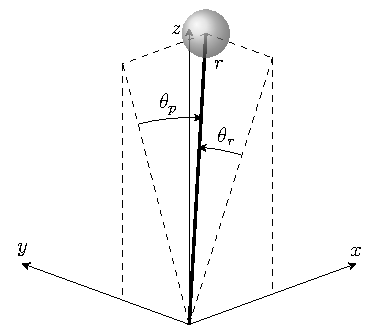
\includegraphics[scale=1.2]{3d_lipm}
  \caption{3D Inverted pendulum model. \label{fig:3d_lipm}}
\end{figure}
\par
The position of the mass point $\vec{p} = \begin{bmatrix} x & y & z \end{bmatrix} \transpose$
is uniquely specified by a set of the Lagrangian coordinates $\vec{q}$
\[
\vec{q} =
\begin{bmatrix}
  \theta_r & \theta_p & r
\end{bmatrix}\transpose
\]
where $r$ is the length of the pendulum while
the angles $\theta_r$ and $\theta_p$ are shown in the Figure \ref{fig:3d_lipm}.
\[
\begin{cases}
  x = r \sine{\theta_p}\\
  y = -r \sine{\theta_r}\\
  z = r \sqrt{1-\sine{\theta_r}^2-\sine{\theta_p}^2}
\end{cases}
\]
In order to develop a model of the pendulum the dynamic equation can be be easily derived
\begin{equation}
  \label{eq:3d_ip_inverseJ}
  m \ddot{\vec{p}} = (J\transpose)^{-1} \vec{\tau}  + m \vec{g}
\end{equation}
where $\vec{g} = \begin{bmatrix} 0 & 0 & -g \end{bmatrix} \transpose$ is the gravity vector,
$\vec{\tau} = \begin{bmatrix} \tau_r & \tau_p & f \end{bmatrix} \transpose$ is the actuated
force/torque vector associated to the Lagrangian coordinates and $J$ is the Jacobian matrix
\[
J = \frac{\partial \vec{p}}{\partial \vec{q}} =
\begin{bmatrix}
  0 & r \cosine{\theta_p} & \sine{\theta_p}\\
  -r\cosine{\theta_r} & 0 & - \sine{\theta_r}\\
  -\frac{r \cosine{\theta_r} \sine{\theta_r}}{\sqrt{1-\sine{\theta_r}^2-\sine{\theta_p}^2}} &   -\frac{r \cosine{\theta_p} \sine{\theta_p}}{\sqrt{1-\sine{\theta_r}^2-\sine{\theta_p}^2}} & \sqrt{1-\sine{\theta_r}^2-\sine{\theta_p}^2}
\end{bmatrix}
\]
In order to erase the term $(J\transpose)^{-1}$ the Equation (\ref{eq:3d_ip_inverseJ})
is multiplied by $J\transpose$
\begin{equation}
  \label{eq:3d_ip}
  m J\transpose \ddot{\vec{p}} = \vec{\tau} + m J\transpose \vec{g}
\end{equation}

\begin{equation}
  \label{eq:3d_ip_expanse}
  m
  \begin{bmatrix}
    0 & -r \cosine{\theta_r} & -\frac{r \cosine{\theta_r} \sine{\theta_r}}{D}\\
    r\cosine{\theta_p} & 0 &-\frac{r \cosine{\theta_p} \sine{\theta_p}}{D}\\
    \sine{\theta_p} & -\sine{\theta_r} & D
  \end{bmatrix}
  \begin{bmatrix}
    \ddot{x}\\
    \ddot{y}\\
    \ddot{z}
  \end{bmatrix} =
  \begin{bmatrix}
    \tau_r\\
    \tau_p\\
    f
  \end{bmatrix}
  - mg
  \begin{bmatrix}
    - r \frac{\cosine{\theta_r} \sine{\theta_r}}{D}\\
    - r \frac{\cosine{\theta_p} \sine{\theta_p}}{D}\\
    D
  \end{bmatrix}
\end{equation}
where $D = \sqrt{1 - \sine{\theta_r} ^ 2 - \sine{\theta_d} ^ 2}$.
\par
Using the first row of the Equation (\ref{eq:3d_ip_expanse}) and multiplying by $D / \cosine{\theta_p}$ the following relation is obtained
\[
\frac{D}{\cosine{\theta_r}} m \left(-\ddot{y} r \cosine{\theta_r} - \ddot{z} r\frac{\cosine{\theta_r}\sine{\theta_r}}{D} \right ) =  \frac{D}{\cosine{\theta_r}} \tau_r + m g r \frac{D}{\cosine{\theta_r}}  \frac{\cosine{\theta_r} \sine{\theta_r}}{D} 
\]
\par
Substituting kinematic relationship in the equation above the equation of the the pendulum along
the \emph{lateral} plane can be obtained
\begin{equation}
  \label{eq:3d_ip_y}
  m(-z \ddot{y} + \ddot{z} y) = \frac{D}{\cosine{\theta_r}} \tau_r - m g y 
\end{equation}
With an analog procedure the equation of the pendulum along the \emph{sagittal} plane can be obtained
\begin{equation}
  \label{eq:3d_ip_x}
  m(z \ddot{x} - \ddot{z} x) = \frac{D}{\cosine{\theta_p}} \tau_d - m g x 
\end{equation}

\subsection{Derivation of the equations of a 3D Linear Inverted Pendulum}
Although the moving pattern of the pendulum has vast possibilities, the class of motion that
would be suitable for walking is selected. In this specific task the trajectory of the pendulum
must lie on a plane characterized by a normal vector
$\begin{bmatrix} k_x & k_y & -1 \end{bmatrix}$
and (passante per il punto) the point $(\begin{matrix} 0 & 0 & z_c \end{matrix})$.
\[
z = k_x x + k_y y + z_c
\]
Substituting the second derivative of the equation above in Equation (\ref{eq:3d_ip_y})
and (\ref{eq:3d_ip_x}) the following system is obtained
\begin{equation}
  \label{eq:3d_lipm}
  \begin{cases}
    \ddot{x} = \frac{g}{z_c}x - \frac{k_y}{z_c}(x \ddot{y} - \ddot{x} y) - \frac{1}{m z_c} u_p\\
    \ddot{y} = \frac{g}{z_c}y - \frac{k_x}{z_c}(x \ddot{y} - \ddot{x} y) - \frac{1}{m z_c} u_r
  \end{cases}
\end{equation}
Where
\[
u_r = \frac{D}{\cosine{\theta_r}} \tau_r \quad u_p = \frac{D}{\cosine{\theta_p}} \tau_p
\]
In the case of the walking on a flat plane (i.e. $k_x = 0$ and $k_y = 0$)
the Equation (\ref{eq:3d_lipm}) becomes
\[
\begin{cases}
  \ddot{x} = \frac{g}{z_c}x - \frac{1}{m z_c} u_p = \frac{g}{z_c} (x - p_x)\\
  \ddot{y} = \frac{g}{z_c}y - \frac{1}{m z_c} u_r = \frac{g}{z_c} (y - p_y)
\end{cases}
\]
where the point $\begin{bmatrix} p_x & p_y & 0 \end{bmatrix}$ is the \emph{Zero Mometum Point} (ZMP).
\par
The set of the equation above can be written in a more elegant form
\[
\ddot{\vec{x}} = \omega^2 (\vec{x} - \vec{p})
\]
where $\vec{x}$ is the vector of the horizontal coordinates of the CoM, while $\vec{p}$ is the vector of $x$ and $y$ position of the ZMP. The parameter $\omega = \sqrt{g/z_c}$ is the time costant of the model.
\par
Since the sagittal and logitudinal dyanamics are complitely decoupled, in the following only the $x$ system is analyzed. The obtained results are valid also for the $y$ dynamics.
\par
The system dynamics of the $x$ coordinate is given by
\begin{equation}
  \label{eq:com_dynamic_equation}
  \dot{\vec{\sigma}} =
  \begin{bmatrix}
    0 & 1 \\
    \omega ^2 &  0
  \end{bmatrix}
  \vec{\sigma} + 
  \begin{bmatrix}
    0\\
    - \omega ^2
\end{bmatrix}
p_x
\end{equation}
where $\vec{\sigma} = \begin{bmatrix} x & \dot{x} \end{bmatrix} \transpose$.
The explicit solution of the dynamics system is
\begin{equation}
  \label{eq:lipm_solution}
  \vec{\sigma}(t) =
  \begin{bmatrix}
    \cosh(\omega t) & \frac{1}{\omega} \sinh(\omega t)\\
    \omega \sinh(\omega t) & \cosh(\omega t)
  \end{bmatrix}
  \vec{\sigma}_0 + 
  \begin{bmatrix}
    1-\cosh(\omega t)\\
    - \omega \sinh(\omega t)
  \end{bmatrix}
  p_x
\end{equation}
where $\vec{\sigma} = \begin{bmatrix} x_0 & \dot{x}_0 \end{bmatrix} \transpose$ is the initial
condition.

\newpage

\section{Capture point}
In this section the concept of Capture point (CP) is introduced.
It is the point on the floor where the robot (modeled as a LIPM) has to step to come
to a complete rest, i.e. the center of mass is exactly located over the ankle and the horizontal
velocity is null.
\par
The concept of Capture point was firstly introduced by Pratt et al. \cite{Pratt2006}
the linear inverted pendulum orbital energy. However, in this report the equations of the CP are
obtained using the explicit solution of the LIP dynamics. The following dissertation will be
mainly based on the work of Englsberger et al. \cite{Englsberger2011}.

\subsection{Derivation of the Capture Point}
The idea is using the Equation (\ref{eq:lipm_solution}) in order to find a point on the ground which, when ZMP is at this position, ensures that the pendulum comes to rest in a vertical position.
\par
More formally the capture point $\xi$ ensures that
\begin{equation}
  \label{eq:cp_condition}
  \begin{cases}
    x \xrightarrow{t\rightarrow \infty} \xi_x\\
    \dot{x} \xrightarrow{t\rightarrow \infty} 0
  \end{cases}
\end{equation}
\par
The Equation (\ref{eq:lipm_solution}) can be written in a more suitable form
\begin{equation}
  \label{eq:lipm_solution_extended}
  \begin{cases}
    x = x_0 \cosh(\omega t) + \frac{\dot{x}_0}{\omega} \sinh(\omega t) + p_x - p_x \cosh(\omega t)\\
    \dot{x} = x_0 \omega \sin(\omega t) + \dot{x}_0 \cosh(\omega t)  - p_x \omega \sinh(\omega t)
  \end{cases}
\end{equation}
Combining the condition (\ref{eq:cp_condition}) and the equation (\ref{eq:lipm_solution_extended})
the following relations can be obtained
\[
\begin{cases}
  p_x = x \big|_{t \rightarrow \infty} = x_0 + \frac{\dot{x}_0}{\omega}\\
  \dot{x} \big|_{t \rightarrow \infty} = x_0 \omega + \dot{x}_0 - p_x \omega = 0
\end{cases}
\]
For a general set of states $\vec{\sigma} = \begin{bmatrix} x & \dot{x} \end{bmatrix} \transpose$
the capture point $\xi_x$ is defined as follow
\begin{equation}
  \label{eq:cp_def}
  \xi_x = x + \frac{\dot{x}}{\omega}
\end{equation}

\subsection{Capture Point dynamics}
In this subsection the dynamic system (\ref{eq:com_dynamic_equation}) is splitted in a stable and
in an unstable parts. The stable one is based on the Capture Point $\xi_x$ and the CoM position $x$, while the unstable part is the dynamics of the Capture Point.
Solving the Equation
(\ref{eq:cp_def}) for $\dot{x}$ the following dynamic system is obtained
\begin{equation}
  \label{eq:com_vs_cp}
  \dot{x} = - \omega (x - \xi_x)
\end{equation}
The position of the CoM $x$ has a stable first order linear dynamics ($\omega > 0$).
The dynamic system of the CP can be obtained by differentiation of (\ref{eq:cp_def}) combined with
the equations (\ref{eq:com_dynamic_equation}) and (\ref{eq:com_vs_cp}).
\begin{equation}
  \label{eq:cp_dynamics}
  \dot{\xi}_x = \dot{x} + \frac{\ddot{x}}{\omega} = \omega (\xi_x - p_x) 
\end{equation}
The obtained dynamic equation has an unstable pole at $\omega$.
\par
By merging the two dynamics systems equations (\ref{eq:com_vs_cp}) and (\ref{eq:cp_dynamics}) a new
formulation of the entire dynamic system can be obtained
\[
\dot{\vec{\theta}} =
\begin{bmatrix}
  -\omega & \omega \\
  0 & \omega
\end{bmatrix}
\vec{\theta} +
\begin{bmatrix}
  0 \\
  -\omega 
\end{bmatrix}
p_x
\]
where the state vector $\vec{\theta}$ is equal to $ \begin{bmatrix} x & \xi_x \end{bmatrix}\transpose$
\newpage
